\chapter{VBTE}
Følgende afsnit beskriver VBTE'ens hardware i de enkelte blokke, grænsefladerne derimellem samt funktionen af blokkene.

\section{Overordnet design}
Nedenfor ses det overordnede hardware blokdiagram. Herefter følger en beskrivelse af de forskellige blokke samt signaler.
\begin{figure}[H]
\centering
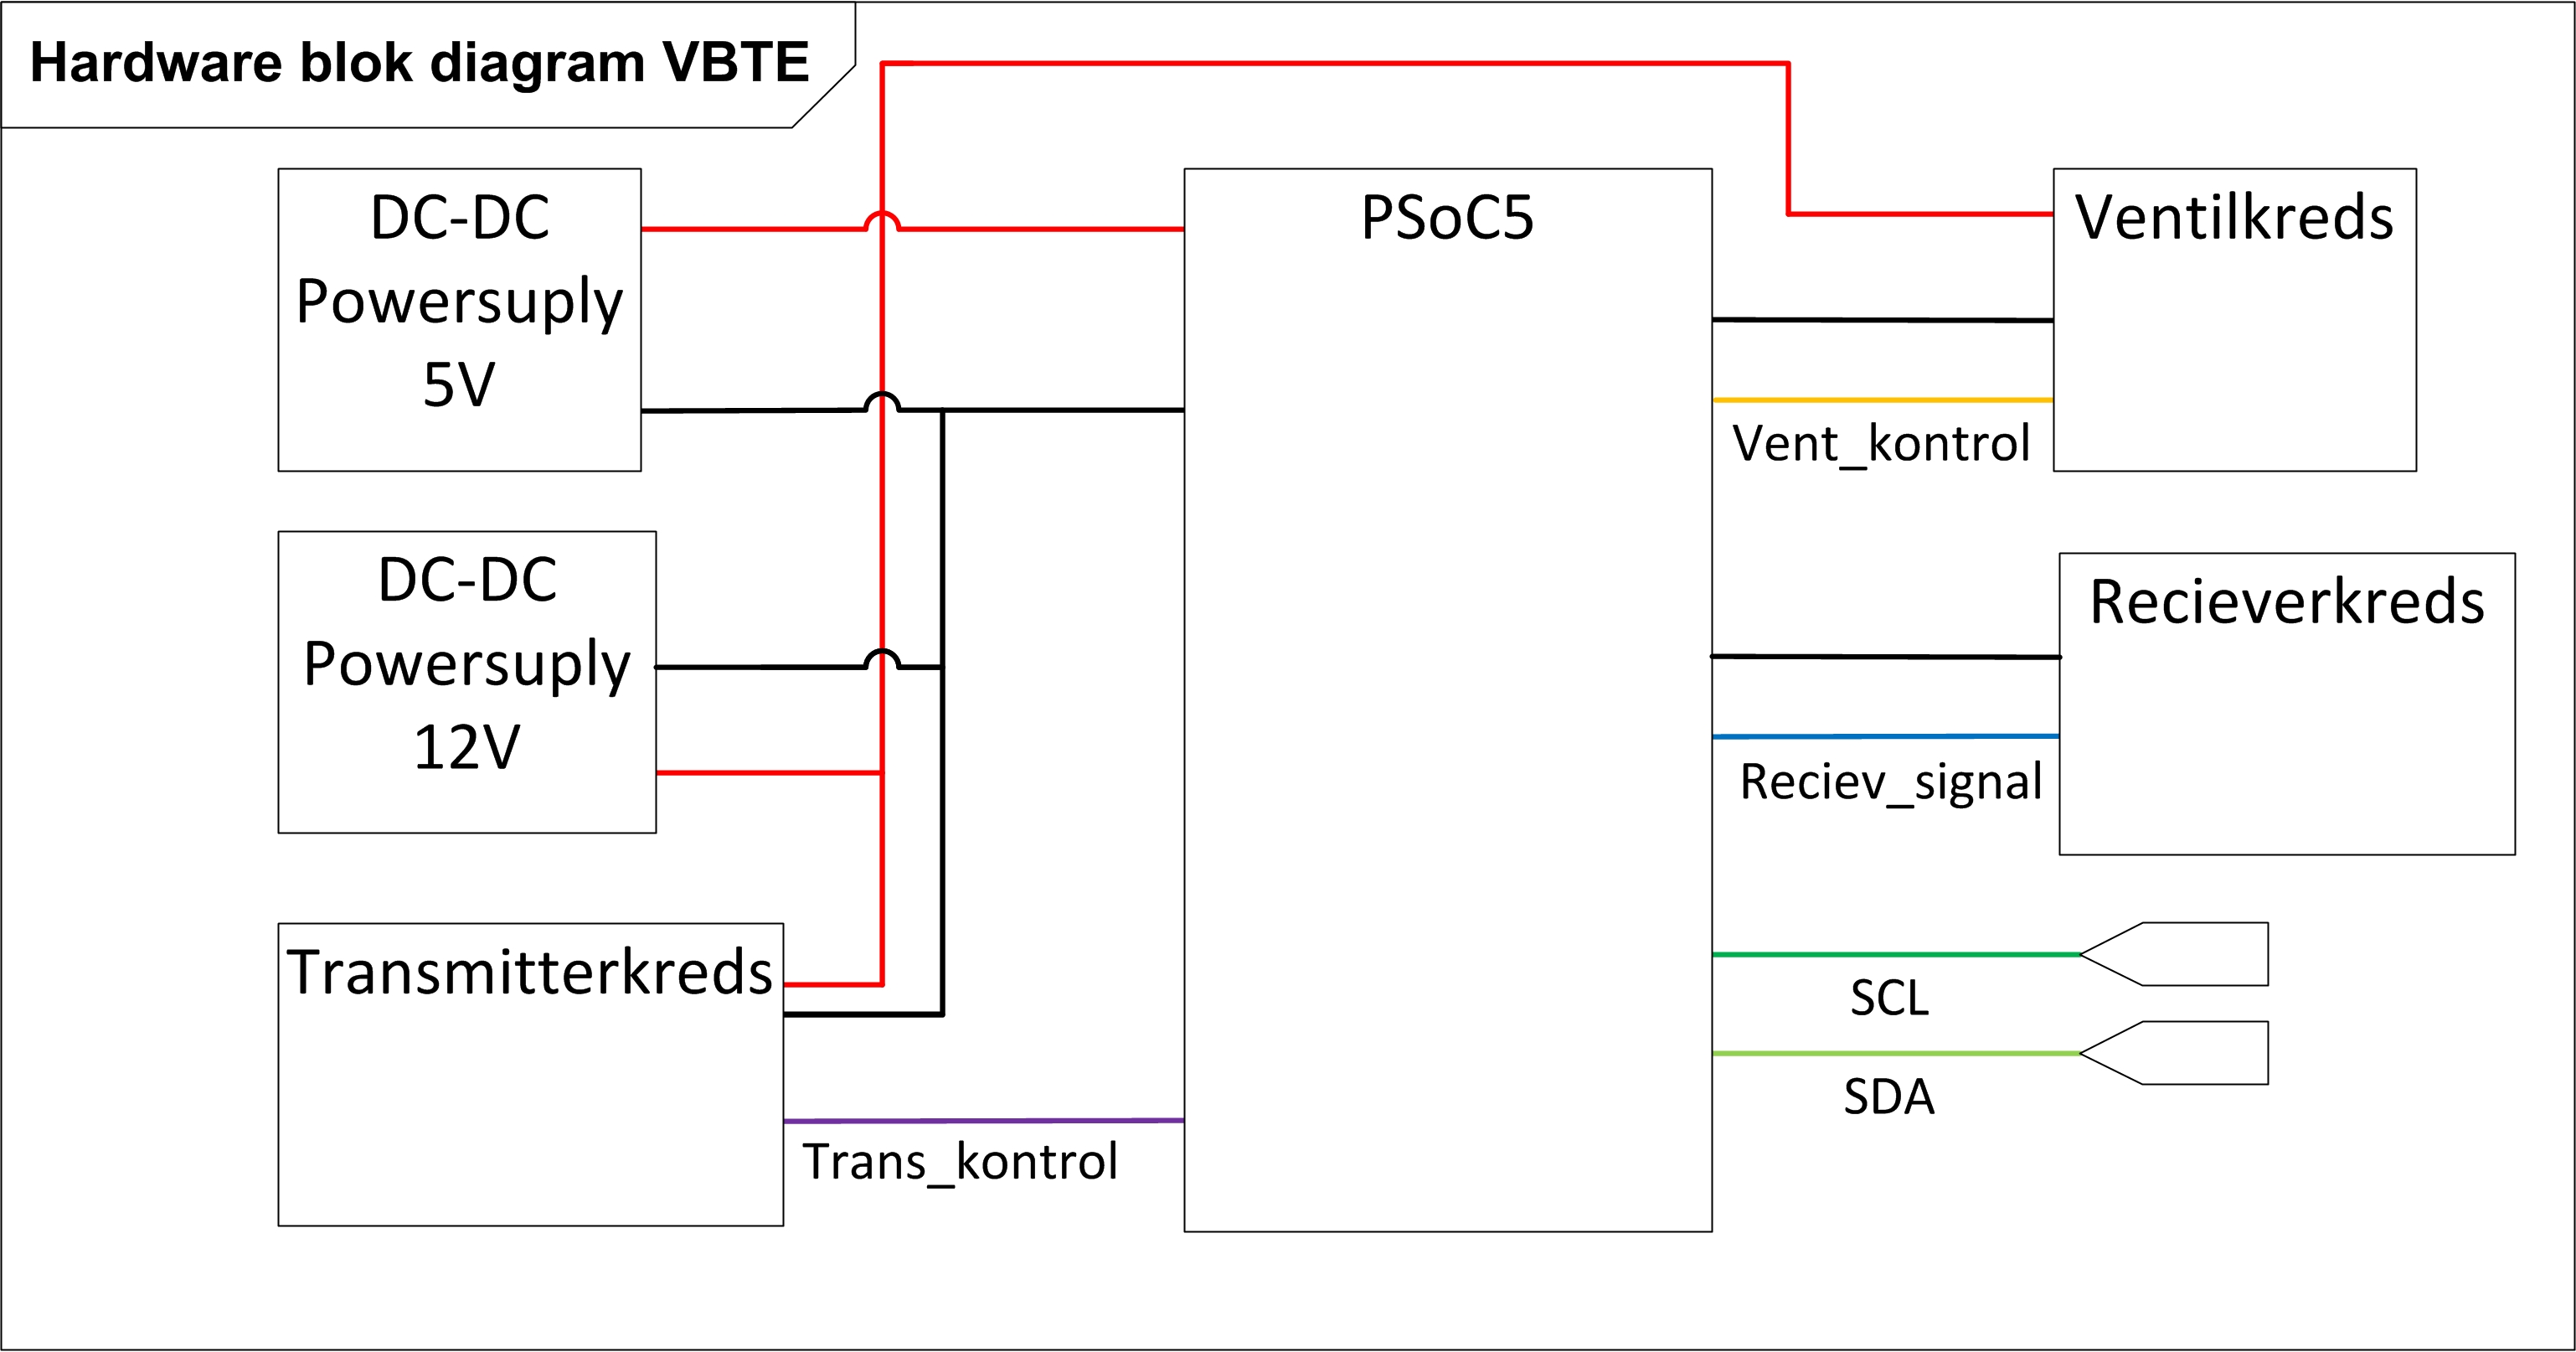
\includegraphics[width=.75\textwidth]{billeder/HWVBTE}
\caption{Overordnet blokdiagram for VBTE hardware}
\label{fig:HWVBTE}
\end{figure}
\subsection{Blokke}
Nedenfor beskrives de enkelte blokke illustreret på \textit{Figur~\ref{fig:HWVBTE}}
\subsubsection{PSoC5}
PSoC'en er den centrale del af VBTE'en og står for styringen af hele VBTE'en. Den består af:
\begin{itemize}
\item MicroController
\item PGA
\item Mixer
\item Timer
\item Clock
\item I2C
\item Delta-Sigma ADC
\item Kontrolregister
\end{itemize}
PSoC'en er et færdigkøbt produkt og for detaljer om de enkelte blokke heri henvises der til databladet for PSoC5.
\subsubsection{DC-DC powersuply 5V}
Se powersuply afsnittet.
\subsubsection{DC-DC powersuply 12V}
Se powersuply afsnittet.
\subsubsection{Transmitterkreds}
Transmitterkredsen består af en MOSFET samt en keramisk ultralyds transmitter(Model: 400ST). Kredsen bliver drevet af 12V powersuply. 
\subsubsection{Reciverkreds}
Recierkredsen består af en keramisk ultralyds reciver(Model: 400SR).
\subsubsection{Ventilkreds}
Ventilkredsen består af en MOSFET samt en ventil(Model: EV210A-1.2 og EV210A-4.5)
\subsubsection{Displaykreds}
Displaykredsen består af et potmeter samt et display af typen WH1602A-YGH-CTK.
\section{Nedbrydning af blokke}
Nedenfor følger nedbrydningen af de enkelte blokke for at beskrive deres opbygning samt grænseflader.
\subsection{PSoC5}
På \textit{Figur \ref{fig:PSoCBlok}} ses HW-designet internt på PSoC'en. De enkelte blokke bliver beskrevet efterfølgende.
\begin{figure}[H]
\centering
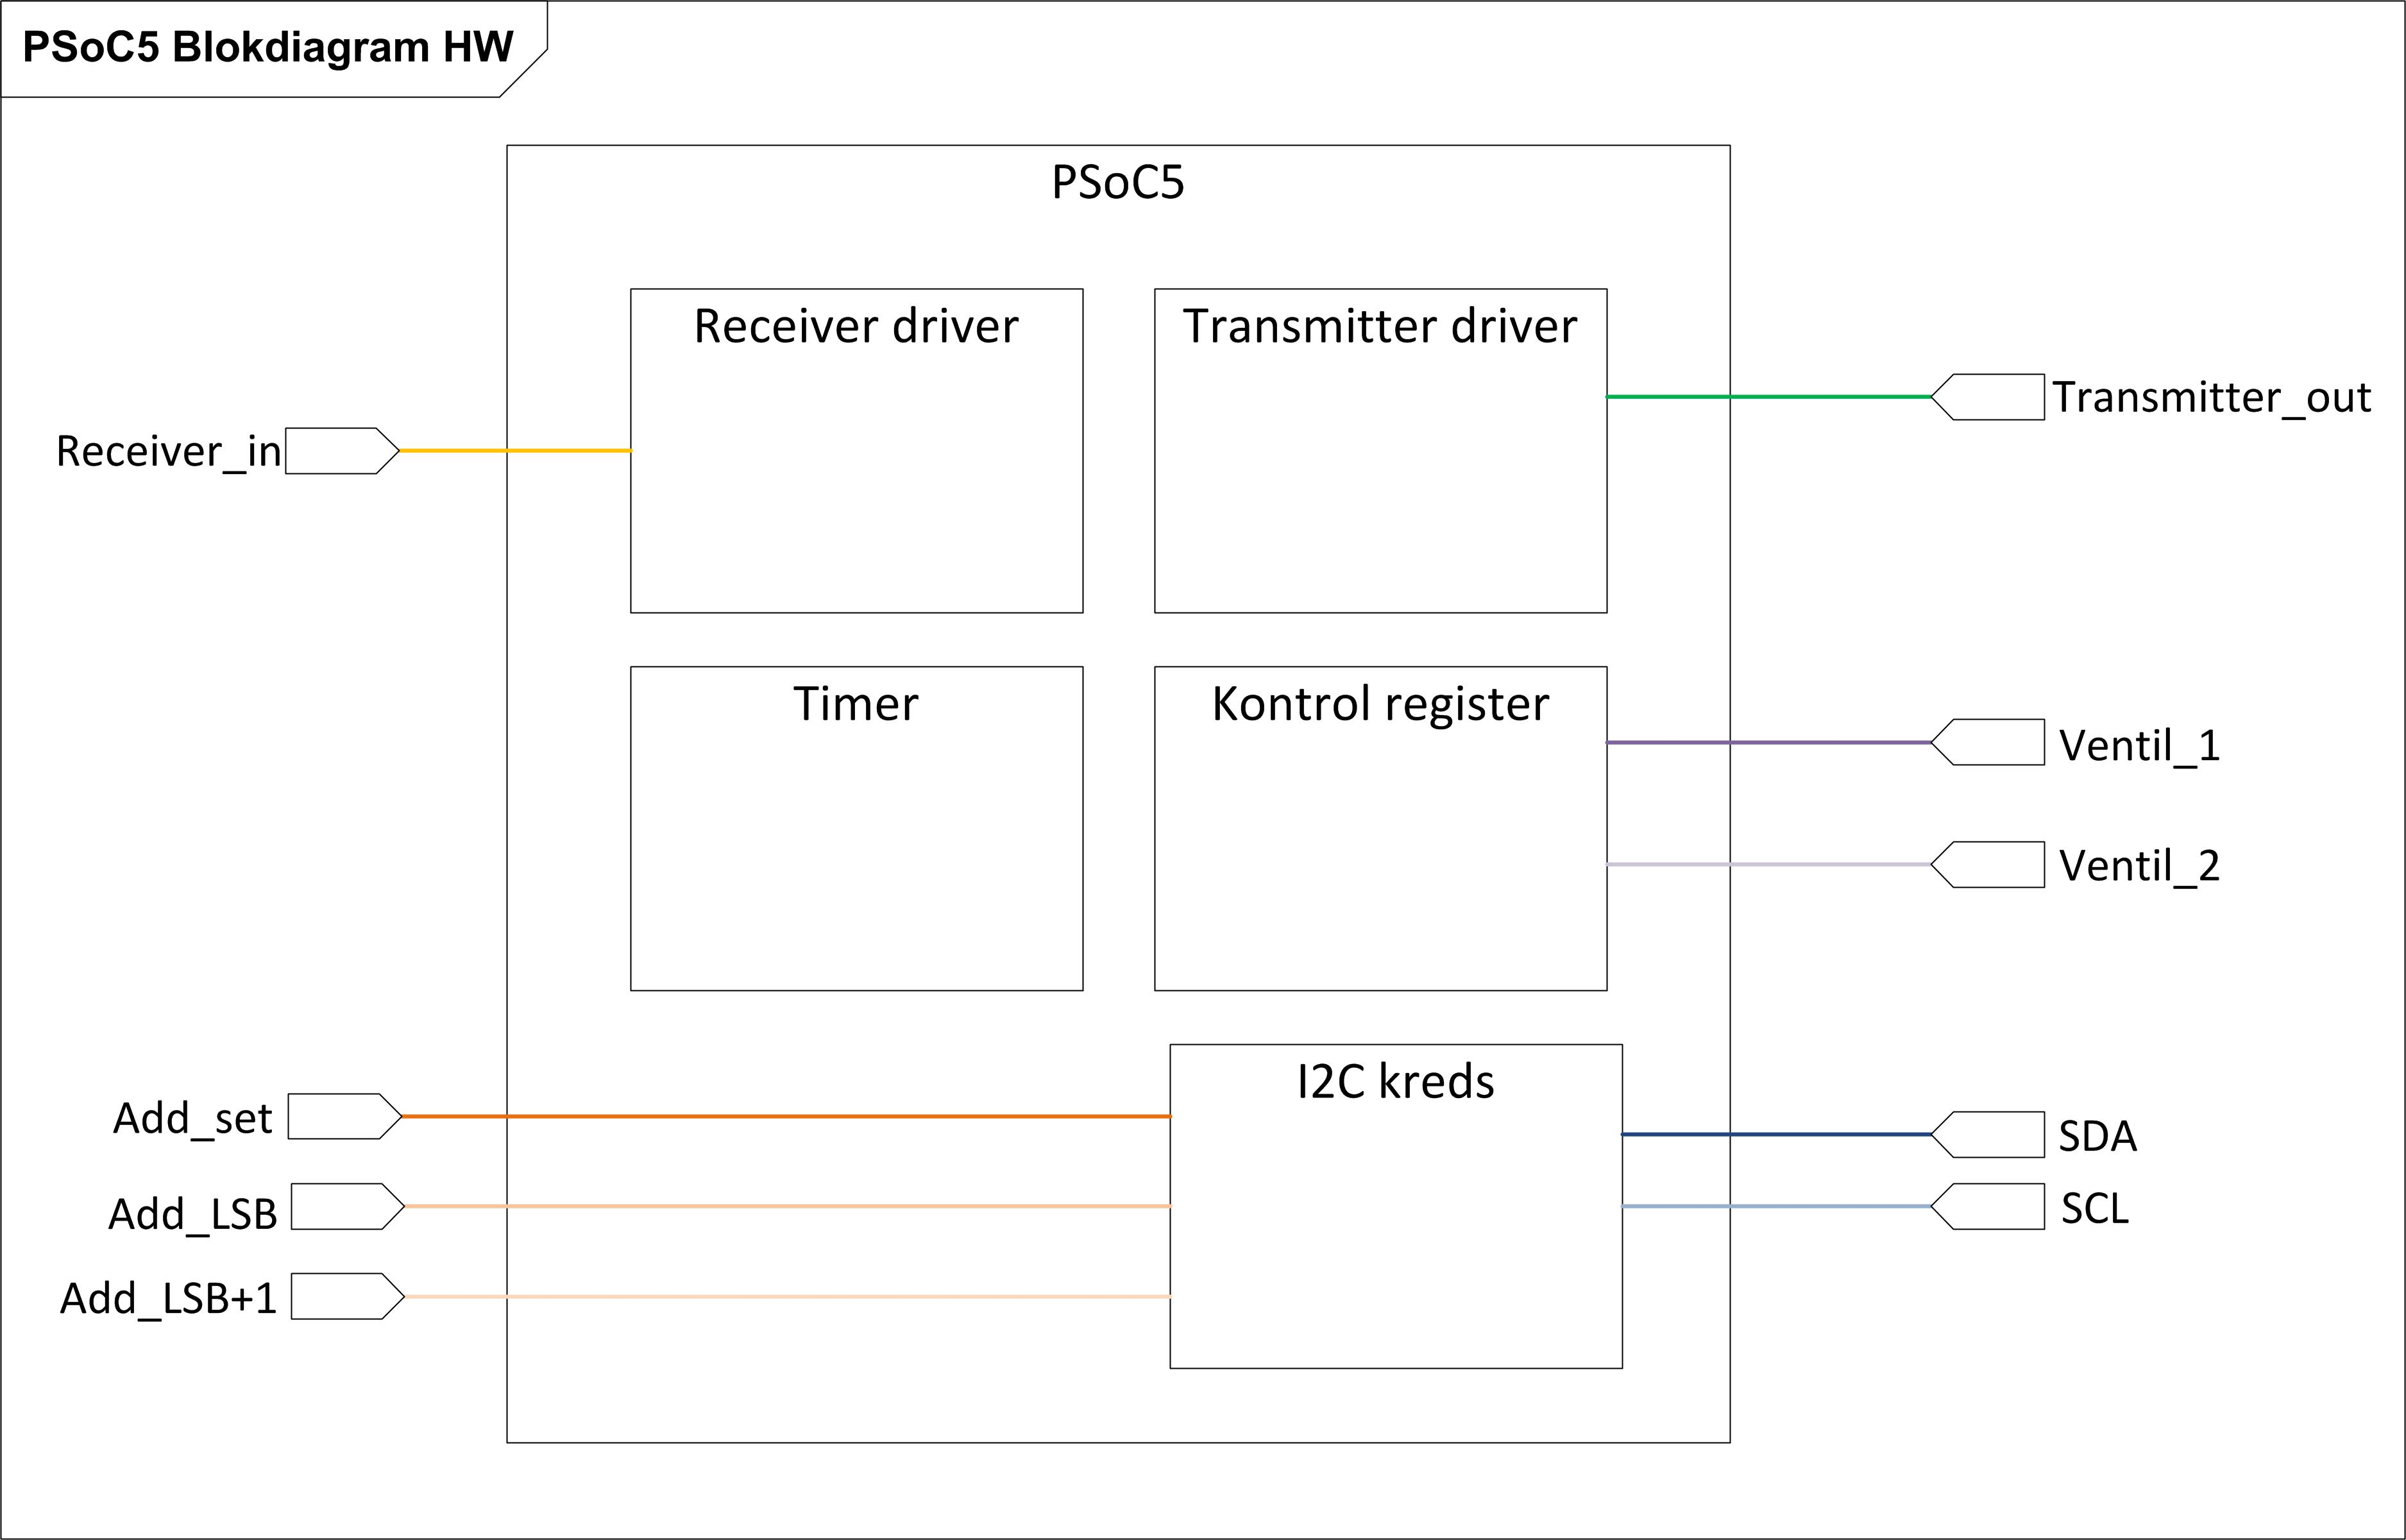
\includegraphics[width=.75\textwidth]{billeder/PSoCBlock}
\caption{PSoC5 blokdiagram}
\label{fig:PSoCBlok}
\end{figure}
\textit{her skal der være en tabel med signalerne og deres spændingsniveauer og hvad de bærer af data}
\subsubsection{Timer}
Beskrivelse af timerblokkens opgave.
\subsubsection{I2C kreds}
Beskrivelse af I2C blokkens opgave samt dets interface.
\subsubsection{LCD Driver}
Beskrivelse af LCD driverens opgave samt dets interface
\subsubsection{Receiver Driver}
Beskrivelse af Receiver driverens opgave samt dets interface
\subsubsection{Transmitter Driver}
Beskrivelse af Transmitter driverens opgave samt dets interface
\subsubsection{Kontrol register}
Beskrivelse af Kontrol registerets opgave samt dets interface.

\subsection{Transmitter kreds}

